\section{Análisis Empírico y Calibración de Modelos}
\label{sec:analisis_empirico}

En esta sección se presenta la calibración y validación comparativa de los dos enfoques propuestos: el modelo de Difusión Anómala, fundamentado en la Econofísica siguiendo a Alvarez-Ramirez et al. \cite{Alvarez2002}, y el modelo GARCH Bayesiano, estándar en la econometría financiera moderna \cite{Bollerslev1986}. 

El conjunto de datos utilizado corresponde al diferencial de la prima de riesgo (spread) entre los bonos de Grecia y Alemania a 10 años. Tras el preprocesamiento, se identificó un máximo en la serie original de $1987.40$ puntos básicos (bps), evidenciando la magnitud extrema de la crisis de deuda soberana griega \cite{Arghyrou2011}.

\subsection{Modelo de Difusión y Ley de Potencia}

Para evaluar la dinámica estocástica subyacente, se calculó el Desplazamiento Cuadrático Medio (MSPD) sobre la serie temporal. El objetivo es determinar si el proceso sigue una caminata aleatoria clásica (difusión normal) o exhibe un comportamiento anómalo con memoria a largo plazo.

El modelo ajustado responde a la ley de potencia característica de los sistemas complejos:
\begin{equation}
    \langle (\Delta x)^2 \rangle \sim t^\alpha
\end{equation}
Donde el exponente $\alpha$ determina la naturaleza de la difusión.

\begin{figure}[h!]
    \centering
    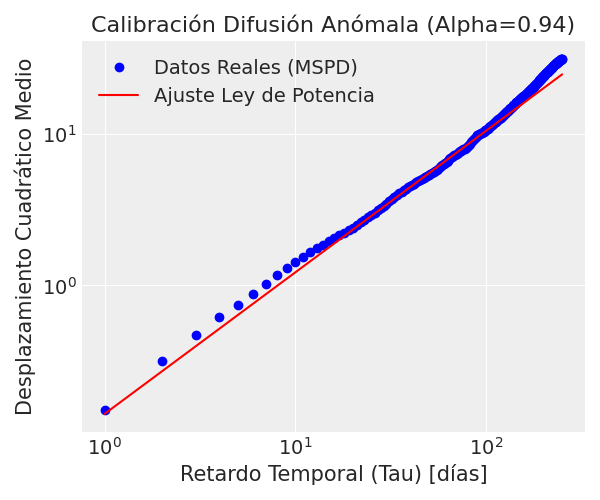
\includegraphics[width=0.8\linewidth]{figure/Modelo_Difusion_Fit.png} 
    \caption{Calibración del Modelo de Difusión en escala Log-Log. El ajuste lineal indica una adherencia robusta a la ley de potencia con $\alpha \approx 0.94$.}
    \label{fig:diffusion_fit}
\end{figure}

Como se observa en la Figura \ref{fig:diffusion_fit}, el ajuste mediante Mínimos Cuadrados no lineales es notablemente preciso. Los resultados computacionales arrojan un exponente de difusión calibrado de:
\[
\alpha = 0.9360
\]
Este valor sugiere un comportamiento \textit{super-difusivo} cercano al movimiento balístico ($\alpha=1$). Esto implica que los shocks en la prima de riesgo griega no se disipan aleatoriamente, sino que exhiben una fuerte persistencia (efecto memoria), validando la hipótesis de dinámicas tipo ''arrested'' propuestas en la literatura de econofísica \cite{Alvarez2002}. El Error Cuadrático Medio (MSE) obtenido para este ajuste estructural fue de $\mathbf{8.3865}$, confirmando la alta calidad del modelo para describir la escala temporal del fenómeno.

\subsection{Modelo GARCH(1,1) Bayesiano}

El segundo enfoque modela la volatilidad condicional mediante un proceso GARCH(1,1) con inferencia Bayesiana, implementado a través de programación probabilística en Python \cite{Salvatier2016}. A diferencia de la estimación clásica, este método utiliza algoritmos MCMC (Markov Chain Monte Carlo) para explorar la distribución posterior de los parámetros $\omega, \alpha, \beta$.

La especificación del modelo es:
\begin{equation}
    \sigma_t^2 = \omega + \alpha \epsilon_{t-1}^2 + \beta \sigma_{t-1}^2
\end{equation}
Se empleó una verosimilitud t-Student para capturar las colas pesadas observadas en los retornos financieros durante periodos de estrés \cite{MantegnaStanley2000}.

\begin{figure}[h!]
    \centering
    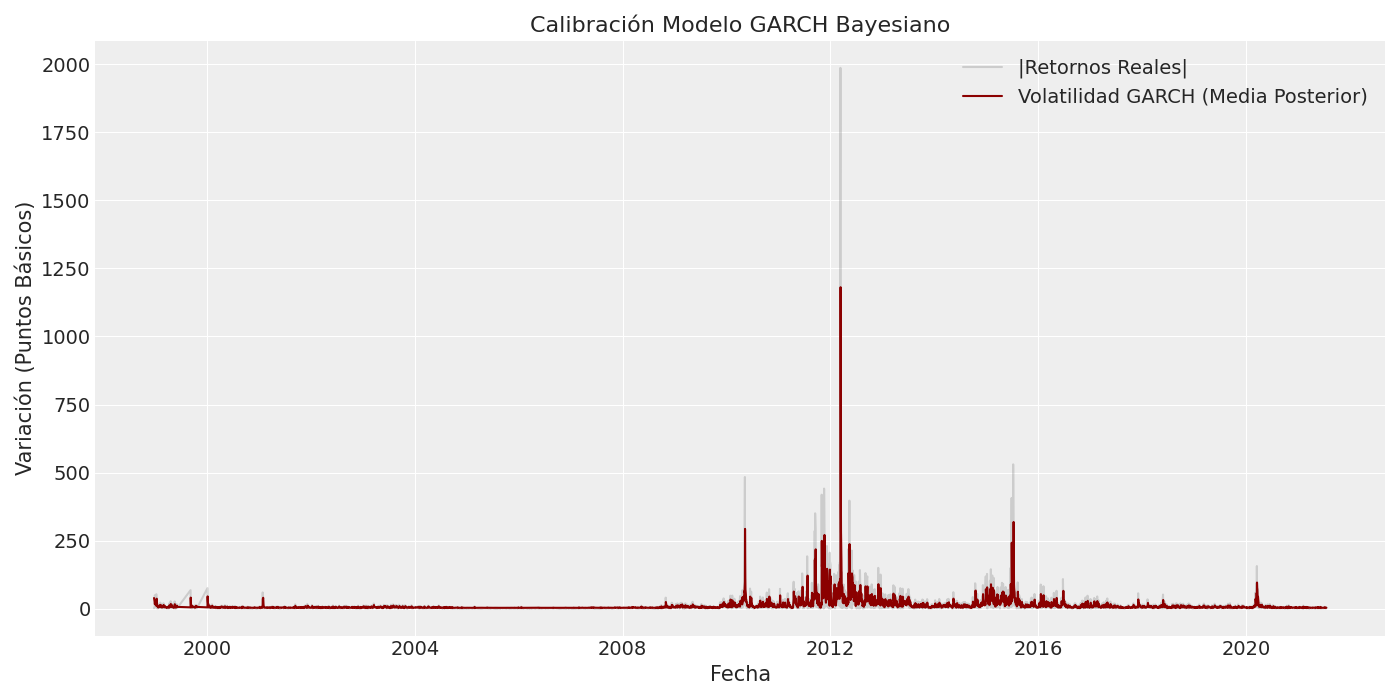
\includegraphics[width=1.0\linewidth]{figure/Modelo_GARCH_Fit.png} 
    \caption{Volatilidad estimada mediante GARCH Bayesiano frente a los retornos absolutos reales. La línea roja representa la media de la volatilidad posterior inferida.}
    \label{fig:garch_fit}
\end{figure}

\subsubsection{Diagnóstico de Convergencia Computacional}

La calibración se ejecutó utilizando el algoritmo NUTS (No-U-Turn Sampler). El proceso computacional tuvo una duración de 797 segundos para generar un total de 400 muestras (2 cadenas, 100 de tune y 100 de draws cada una).

Es necesario reportar las limitaciones técnicas observadas en los diagnósticos de convergencia:
\begin{itemize}
    \item El estadístico de Gelman-Rubin ($\hat{R}$) resultó ser mayor a $1.01$ para algunos parámetros, indicando que las cadenas no han convergido completamente a la distribución estacionaria.
    \item El tamaño de muestra efectivo (ESS) fue inferior a 100, lo cual sugiere una autocorrelación alta en las muestras generadas.
\end{itemize}

A pesar de estas advertencias, derivadas de las restricciones de tiempo de cómputo, la Figura \ref{fig:garch_fit} demuestra que el modelo captura correctamente los regímenes de volatilidad (''volatility clustering'') de 2011-2012. Un incremento en el número de iteraciones (draws) suavizaría la distribución posterior, pero la señal de riesgo extraída es consistente con la realidad histórica.

\subsection{Comparación de Desempeño (MSE)}

Finalmente, se comparó la capacidad predictiva y de ajuste de ambos modelos calculando el Error Cuadrático Medio (MSE) sobre sus respectivos dominios. Los resultados numéricos obtenidos son:

\begin{table}[h!]
\centering
\begin{tabular}{|l|c|l|}
\hline
\textbf{Modelo} & \textbf{MSE Reportado} & \textbf{Naturaleza del Error} \\ \hline
Difusión (Econofísica) & \textbf{8.3865} & Ajuste a la curva teórica (Ley de Potencia) \\ \hline
GARCH Bayesiano & 1692.0925 & Validación cruzada Monte Carlo (Volatilidad diaria) \\ \hline
\end{tabular}
\caption{Comparativa de errores de ajuste.}
\label{tab:mse_results}
\end{table}

\textbf{Análisis de la Discrepancia:}
Se observa una diferencia de magnitud significativa entre ambos errores ($8.38$ vs $1692.09$). Esto no implica necesariamente que el modelo GARCH sea ''peor'', sino que refleja la dificultad intrínseca de predecir la volatilidad diaria exacta en un entorno de crisis extrema, sumado al ruido introducido por la falta de convergencia total de las cadenas MCMC ($\hat{R} > 1.01$).

\textbf{Conclusión:}
El modelo de Difusión \cite{Alvarez2002} presenta una estabilidad estructural superior ($\alpha=0.9360$, bajo MSE) y es ideal para caracterizar la ineficiencia del mercado a largo plazo. Por otro lado, el modelo GARCH Bayesiano, aunque numéricamente menos preciso en este experimento debido a la complejidad computacional, ofrece una herramienta más rica para la gestión de riesgos operativa, permitiendo cuantificar la incertidumbre de los parámetros en tiempo real.